%%%%%%%% ICML 2025 PAPER: AdaDMD %%%%%%%%%%%%%%%%%

\documentclass{article}

\usepackage{microtype}
\usepackage{graphicx}
\usepackage{subfigure}
\usepackage{booktabs}
\usepackage{hyperref}

\newcommand{\theHalgorithm}{\arabic{algorithm}}

\usepackage[accepted]{icml2025}

\usepackage{amsmath}
\usepackage{amssymb}
\usepackage{mathtools}
\usepackage{amsthm}
\usepackage[capitalize,noabbrev]{cleveref}
\usepackage{algorithm}
\usepackage{algorithmic}
\usepackage{xcolor}
\usepackage{multirow}

%%%%%%%%%%%%%%%%%%%%%%%%%%%%%%%%
% THEOREMS
%%%%%%%%%%%%%%%%%%%%%%%%%%%%%%%%
\theoremstyle{plain}
\newtheorem{theorem}{Theorem}[section]
\newtheorem{proposition}[theorem]{Proposition}
\theoremstyle{remark}
\newtheorem{remark}[theorem]{Remark}

%%%%%%%%%%%%%%%%%%%%%%%%%%%%%%%%
% CUSTOM COMMANDS
%%%%%%%%%%%%%%%%%%%%%%%%%%%%%%%%
\newcommand{\R}{\mathbb{R}}
\newcommand{\E}{\mathbb{E}}
\newcommand{\KL}{\mathrm{KL}}
\newcommand{\bx}{\mathbf{x}}
\newcommand{\bz}{\mathbf{z}}
\newcommand{\bepsilon}{\boldsymbol{\epsilon}}
\newcommand{\btheta}{\boldsymbol{\theta}}
\newcommand{\bphi}{\boldsymbol{\phi}}
\newcommand{\bpsi}{\boldsymbol{\psi}}

\icmltitlerunning{AdaDMD: Adaptive Distribution Matching Distillation}

\begin{document}

\twocolumn[
\icmltitle{AdaDMD: Adaptive Distribution Matching Distillation\\via Low-Rank Score Estimation and Learned Density-Ratio Weighting\thanks{Code: \url{https://github.com/ramzzes13/onestepdiff}}}

\icmlsetsymbol{equal}{*}

\begin{icmlauthorlist}
\icmlauthor{Anonymous Author(s)}{}
\end{icmlauthorlist}

\icmlkeywords{Diffusion Models, Knowledge Distillation, One-Step Generation, Distribution Matching, LoRA}

\vskip 0.3in
]

\printAffiliationsAndNotice{}

% ============================================================
\begin{abstract}
Distribution Matching Distillation (DMD) enables single-step image generation by minimizing the KL divergence between generator and data distributions through dual score functions. However, DMD requires maintaining three full diffusion models simultaneously, demanding extreme GPU memory (72 A100s for text-to-image training) and making the approach inaccessible to most researchers. We propose \textbf{AdaDMD}, which addresses this through three contributions: (1) replacing the full-copy fake score model with a LoRA adapter, reducing memory by approximately 60\%; (2) learning adaptive timestep weights via a density-ratio estimator trained with noise contrastive estimation, replacing fixed heuristic weighting; and (3) using the learned density ratio as both a training regularizer and an inference-time sample verifier. On CIFAR-10 distillation with a pretrained DDPM teacher, AdaDMD trains on a single GPU using under 1\,GB. Combined with paired LPIPS regression loss to prevent mean collapse, AdaDMD achieves \textbf{110.38 FID} (with DR-8 verification), a 50\% improvement over the MSE-based distillation baseline. A key finding is that maintaining constant regression weight throughout training is critical---decaying it causes FID degradation of 25+ points. Ablation studies confirm that adaptive weighting improves FID by 2.1 points, and the density-ratio verifier provides up to 4.6 FID points improvement at inference time.\footnote{Code: \texttt{github.com/ramzzes13/onestepdiff}}
\end{abstract}

% ============================================================
\section{Introduction}
\label{sec:intro}

Diffusion models~\citep{ho2020denoising, song2021scorebased} generate high-fidelity images through iterative denoising, typically requiring 20--1000 network evaluations. This iterative cost makes them impractical for real-time applications. Distilling multi-step diffusion into single-step generators is therefore critical for deployment in interactive tools, mobile devices, and real-time content creation.

Distribution Matching Distillation (DMD)~\citep{yin2024onestep} introduced an effective framework for this: minimize the KL divergence between generated and real distributions by expressing its gradient as the difference of two score functions---one from a frozen pretrained model (real score) and one from a dynamically updated copy (fake score). Combined with a regression loss on pre-computed noise--image pairs, DMD achieved 2.62 FID on ImageNet 64$\times$64 in a single step.

DMD2~\citep{yin2024dmd2} improved this by eliminating the regression loss through a two-time-scale update rule and adding a GAN discriminator, reaching 1.28 FID on ImageNet 64$\times$64. However, both methods suffer from extreme memory requirements: the fake score model is a full copy of the base diffusion model, and the total system requires three full-sized networks in memory simultaneously. DMD's text-to-image experiments required 72 A100 GPUs.

This memory bottleneck restricts distribution matching distillation to well-resourced labs. Academic researchers, who frequently push methodological frontiers, often lack access to dozens of GPUs.

We propose \textbf{AdaDMD} (Adaptive Distribution Matching Distillation), which makes three modifications to the DMD framework:

\begin{enumerate}
\item \textbf{LoRA-based fake score estimation.} We replace the full-copy fake score model with a low-rank adaptation (LoRA)~\citep{hu2022lora} of the frozen pretrained model. Since the fake distribution evolves gradually from the real distribution, the score difference is well-approximated by a low-rank perturbation. A rank-8 adapter adds only 2.9\% parameters, reducing memory by approximately 60\%.

\item \textbf{Learned density-ratio weighting.} We replace DMD's fixed timestep weighting heuristic with adaptive weights derived from a lightweight density-ratio estimator trained via noise contrastive estimation~\citep{gutmann2010noise}. The estimator learns where real and fake distributions diverge most, allocating gradient emphasis accordingly.

\item \textbf{Density-ratio regularization and verification.} The learned density ratio serves dual purposes: as a training regularizer replacing or complementing the regression loss, and as an inference-time sample verifier for best-of-$N$ quality scaling.
\end{enumerate}

We validate AdaDMD on CIFAR-10 32$\times$32 distillation using a pretrained DDPM teacher~\citep{ho2020denoising}. Training requires under 1\,GB of GPU memory on a single device. Ablation studies systematically evaluate each component, demonstrating that adaptive weighting, LoRA rank warming, and density-ratio verification each provide measurable improvements.

% ============================================================
\section{Related Work}
\label{sec:related}

\paragraph{Distribution matching distillation.}
DMD~\citep{yin2024onestep} framed one-step distillation as minimizing the KL divergence between generated and real distributions, using the gradient identity $\nabla_{\bx} \KL(p_{\text{fake}} \| p_{\text{real}}) \propto s_{\text{fake}}(\bx_t, t) - s_{\text{real}}(\bx_t, t)$ where $s$ denotes score functions. A regression loss on teacher-generated pairs stabilizes training. DMD2~\citep{yin2024dmd2} removed the regression loss via two-time-scale updates and added a GAN discriminator, improving FID from 2.62 to 1.28 on ImageNet 64$\times$64. Both methods require multiple full diffusion model copies in memory.

\paragraph{Consistency-based methods.}
Consistency Models~\citep{song2023consistency} enforce self-consistency along the probability flow ODE trajectory. Latent Consistency Models (LCM)~\citep{luo2023latent} adapted this to latent diffusion, and LCM-LoRA~\citep{luo2023lcmlora} showed that LoRA adapters can serve as universal acceleration modules. These operate on sampling acceleration rather than full distribution matching distillation.

\paragraph{Adversarial distillation.}
Adversarial Diffusion Distillation~\citep{sauer2023adversarial} combined score distillation with adversarial training for real-time generation. Score Identity Distillation~\citep{zhou2024score} achieved exponentially fast distillation by leveraging score identities on semi-implicit distributions.

\paragraph{Progressive and simplified distillation.}
Progressive Distillation~\citep{salimans2022progressive} halves the number of sampling steps iteratively. InstaFlow~\citep{liu2023instaflow} used rectified flow for one-step text-to-image generation. SwiftBrush~\citep{nguyen2024swiftbrush} applied variational score distillation.

\paragraph{Memory-efficient approaches.}
LCM-LoRA~\citep{luo2023lcmlora} demonstrated LoRA-based few-step sampling with minimal fine-tuning, though for sampling acceleration rather than distribution matching. Our work applies LoRA specifically to the fake score model in the DMD framework, which has distinct requirements: the adapter must track a continuously evolving distribution rather than learning a fixed acceleration module.

\paragraph{Low-rank adaptation.}
LoRA~\citep{hu2022lora} parameterizes weight updates as low-rank decompositions $\Delta W = BA$ where $B \in \R^{d \times r}$ and $A \in \R^{r \times k}$ with $r \ll \min(d, k)$. Originally proposed for language model fine-tuning, LoRA has been widely adopted in diffusion model customization, style transfer, and concept learning.

% ============================================================
\section{Method}
\label{sec:method}

\subsection{Background: Distribution Matching Distillation}
\label{sec:background}

A diffusion model defines a forward process that adds Gaussian noise to data $\bx_0 \sim p_{\text{data}}$:
\begin{equation}
q(\bx_t | \bx_0) = \mathcal{N}(\bx_t; \sqrt{\bar\alpha_t}\, \bx_0, (1 - \bar\alpha_t)\mathbf{I})
\label{eq:forward}
\end{equation}
where $\bar\alpha_t = \prod_{s=1}^t (1 - \beta_s)$ and $\{\beta_t\}$ is the noise schedule. A denoising model $\bepsilon_{\btheta}(\bx_t, t)$ is trained to predict the added noise.

DMD~\citep{yin2024onestep} trains a single-step generator $G_{\btheta}: \bz \mapsto \bx_{\text{fake}}$ by minimizing:
\begin{equation}
\mathcal{L}_{\text{DMD}} = \E_t\left[w_t \cdot \nabla_{G_{\btheta}(\bz)} \KL\bigl(p_{\text{fake},t} \,\|\, p_{\text{real},t}\bigr)\right]
\label{eq:dmd}
\end{equation}
The gradient of this KL divergence decomposes as:
\begin{equation}
\nabla_{\bx} \KL = \bepsilon_{\bphi}^{\text{fake}}(\bx_t, t) - \bepsilon_{\btheta}^{\text{real}}(\bx_t, t)
\label{eq:score_diff}
\end{equation}
where $\bepsilon^{\text{real}}$ is the frozen pretrained model and $\bepsilon^{\text{fake}}_{\bphi}$ is a copy of the pretrained model fine-tuned on generator outputs. The weighting $w_t = \sigma_t^2 / \alpha_t$ with gradient normalization~\citep{yin2024onestep} balances contributions across noise levels.

\subsection{LoRA-Based Fake Score Estimation}
\label{sec:lora_score}

The fake score model $\bepsilon^{\text{fake}}_{\bphi}$ in DMD is initialized from the pretrained model and continuously updated to track the generator's distribution. Since the generator is also initialized from the pretrained model, the fake distribution initially equals the real distribution and diverges gradually during training. The score difference $\bepsilon^{\text{fake}} - \bepsilon^{\text{real}}$ is therefore small early in training and grows slowly.

This motivates a low-rank parameterization. We replace $\bepsilon^{\text{fake}}_{\bphi}$ with:
\begin{equation}
\bepsilon^{\text{fake}}(\bx_t, t) = \bepsilon^{\text{real}}(\bx_t, t; W + \Delta W_{\text{LoRA}})
\label{eq:lora_score}
\end{equation}
where $\Delta W_{\text{LoRA}} = BA$ with $B \in \R^{d \times r}$, $A \in \R^{r \times k}$, applied to attention and convolution layers. We use PEFT~\citep{hu2022lora} LoRA adapters on the frozen base model, targeting query, key, value, output projections, and convolution layers.

\paragraph{Rank warming.} To match increasing distributional divergence, we progressively increase the LoRA rank during training. Starting from rank $r_0$, we double it every $K$ steps up to $r_{\max}$:
\begin{equation}
r(t) = \min\bigl(r_0 \cdot 2^{\lfloor t / K \rfloor},\, r_{\max}\bigr)
\end{equation}
New rank components are zero-initialized, preserving the current adapter behavior while adding capacity.

\paragraph{Memory analysis.} For the HuggingFace DDPM-CIFAR10-32 model (35.7M parameters), a rank-8 LoRA adapter adds 1.08M parameters (2.9\% of base). The full fake score copy requires 35.7M parameters. Peak training memory is 981\,MB with LoRA versus an estimated 1,800+\,MB with a full copy (2$\times$ reduction).

\subsection{Learned Density-Ratio Weighting}
\label{sec:density_ratio}

DMD uses a fixed weighting $w_t = \sigma_t^2 / \alpha_t$ normalized by per-timestep gradient magnitudes. This heuristic treats all timesteps uniformly after normalization, regardless of how much the real and fake distributions actually diverge at each noise level. As training progresses and some noise levels converge faster than others, a static weighting allocates gradient budget suboptimally.

We introduce a lightweight density-ratio network $r_{\bpsi}(\bx_t, t)$ that estimates $\log\frac{p_{\text{fake},t}(\bx_t)}{p_{\text{real},t}(\bx_t)}$. This network is trained via binary classification (noise contrastive estimation):
\begin{equation}
\mathcal{L}_{\text{NCE}} = -\E_{\bx_t \sim p_{\text{real},t}}\!\bigl[\log \sigma(r_{\bpsi})\bigr] - \E_{\bx_t \sim p_{\text{fake},t}}\!\bigl[\log(1 - \sigma(r_{\bpsi}))\bigr]
\label{eq:nce}
\end{equation}
where $\sigma$ is the sigmoid function, real noised samples are constructed from training data, and fake noised samples from generator outputs.

The adaptive weight at timestep $t$ is:
\begin{equation}
w_t^{\text{ada}} = \frac{\sigma_t^2}{\alpha_t} \cdot \frac{1}{\text{EMA}(|r_{\bpsi}(\bx_t, t)|) + \epsilon}
\label{eq:ada_weight}
\end{equation}
This downweights timesteps where the density-ratio magnitude is large (indicating large distributional mismatch already receiving strong gradients) and upweights timesteps where the ratio is small (indicating potential areas of undertrained alignment).

\paragraph{Architecture.} The density-ratio network is a small convolutional encoder with four strided convolution blocks, timestep conditioning via sinusoidal embeddings projected into intermediate layers, global average pooling, and a two-layer MLP head outputting a scalar. Total: 320K parameters (0.9\% of the base model).

\subsection{Density-Ratio Regularization}
\label{sec:dr_reg}

DMD uses a regression loss $\|\text{LPIPS}(G_{\btheta}(\bz_i), \bx_i^{\text{teacher}})\|$ on pre-computed noise--image pairs from the teacher to prevent mode collapse. This requires expensive offline generation of teacher samples.

We propose a density-ratio regularizer as an alternative:
\begin{equation}
\mathcal{L}_{\text{DR}} = \E_{\bz}\bigl[\max(0, -r_{\bpsi}(G_{\btheta}(\bz), 0) + \delta)\bigr]
\label{eq:dr_loss}
\end{equation}
where $\delta$ is a margin and $r_{\bpsi}(\cdot, 0)$ evaluates the density ratio at $t = 0$ (clean images). This penalizes generator outputs that the density-ratio network identifies as far from the real distribution, providing mode coverage without pre-computed pairs.

The total generator loss combines the adaptive DM loss with regularization:
\begin{equation}
\mathcal{L}_{\text{total}} = \lambda_{\text{DM}} \mathcal{L}_{\text{DM}}^{\text{ada}} + \lambda_{\text{reg}} \mathcal{L}_{\text{reg}} + \lambda_{\text{DR}} \mathcal{L}_{\text{DR}}
\label{eq:total_loss}
\end{equation}
where $\mathcal{L}_{\text{reg}}$ is the paired LPIPS regression loss (when available) with a decaying weight schedule.

\subsection{Inference-Time Density-Ratio Verification}
\label{sec:dr_verify}

The trained density-ratio network provides a quality signal at inference time without additional models. Given $N$ candidate generations $\{G_{\btheta}(\bz_1), \ldots, G_{\btheta}(\bz_N)\}$ for a single sample, we select:
\begin{equation}
\bx^* = \arg\min_{i} r_{\bpsi}(G_{\btheta}(\bz_i), 0)
\label{eq:verify}
\end{equation}
selecting the candidate most consistent with the real distribution. This provides a principled quality--latency tradeoff controlled by $N$.

\subsection{Training Algorithm}
\label{sec:algorithm}

\begin{algorithm}[t]
\caption{AdaDMD Training}
\label{alg:adadmd}
\begin{algorithmic}[1]
\REQUIRE Pretrained model $\bepsilon^{\text{real}}$, dataset $\mathcal{D}$
\STATE Init $G_{\btheta} \leftarrow \bepsilon^{\text{real}}$ (weights)
\STATE Init LoRA adapter $\Delta_{\bphi}$ with rank $r_0$
\STATE Init density-ratio network $r_{\bpsi}$
\FOR{step $= 1, \ldots, T$}
    \STATE $\bz \sim \mathcal{N}(0, \mathbf{I})$, $\bx_{\text{real}} \sim \mathcal{D}$
    \STATE $\bx_{\text{fake}} \leftarrow G_{\btheta}(\bz)$
    \STATE \textit{// Update LoRA fake score}
    \STATE Sample $t$; $\bx_t \leftarrow q(\bx_{\text{fake}}, t)$
    \STATE $\mathcal{L}_{\text{LoRA}} \leftarrow \|\bepsilon^{\text{real}}(\bx_t, t; W + \Delta_{\bphi}) - \bepsilon\|^2$
    \STATE Update $\bphi$
    \STATE \textit{// Update density-ratio}
    \STATE $\mathcal{L}_{\text{NCE}}$ from noised real/fake (Eq.~\ref{eq:nce})
    \STATE Update $\bpsi$
    \STATE \textit{// Update generator}
    \STATE $w_t^{\text{ada}}$ from Eq.~\ref{eq:ada_weight}
    \STATE $\mathcal{L}_{\text{total}}$ from Eq.~\ref{eq:total_loss}
    \STATE Update $\btheta$; EMA update
    \IF{step mod $K = 0$ and $r < r_{\max}$}
        \STATE $r \leftarrow \min(2r, r_{\max})$
    \ENDIF
\ENDFOR
\end{algorithmic}
\end{algorithm}

% ============================================================
\section{Experiments}
\label{sec:experiments}

\subsection{Setup}

\paragraph{Base model and dataset.}
We distill the publicly available \texttt{google/ddpm-cifar10-32} model from HuggingFace (35.7M parameters, trained by~\citet{ho2020denoising}). Training and evaluation use CIFAR-10~\citep{krizhevsky2009learning} at 32$\times$32 resolution with the standard 50K training / 10K test split.

\paragraph{Teacher pair generation.}
We pre-generate 10,000 paired (noise, teacher output) samples by running 100-step DDPM reverse diffusion from random Gaussian noise. These pairs provide regression targets for the LPIPS loss.

\paragraph{Training details.}
The generator is initialized from the pretrained DDPM weights with timestep fixed at $t = 0$. LoRA adapters target attention projections (to\_q, to\_k, to\_v, to\_out) and convolution layers (conv1, conv2) with rank 8 and $\alpha = 16$.

Training uses AdamW~\citep{loshchilov2019decoupled} with learning rates $2 \times 10^{-5}$ (generator), $10^{-4}$ (LoRA), $10^{-4}$ (density-ratio), and batch size 8. Two-phase training: 5,000 steps of regression-only (LPIPS on teacher pairs), then 45,000 steps of combined DM + regression + DR losses. Regression weight decays linearly from 1.0 to 0.3 during Phase 2. DM loss is scaled by $\lambda_{\text{DM}} = 10^{-4}$.

All experiments run on a single GPU with peak memory under 1\,GB.

\paragraph{Evaluation.}
FID~\citep{heusel2017gans} is computed between 5,000 generated samples and the CIFAR-10 test set using Inception v3 features. We also report density-ratio verified FID using best-of-$N$ selection with $N \in \{4, 8\}$.

\paragraph{Ablations.}
Ablation studies use a custom SmallUNet (6.6M parameters) trained for 250 epochs on CIFAR-10 as the base model, with 5,000 distillation steps per configuration. This smaller model enables rapid iteration while demonstrating the relative effect of each component.

\subsection{Ablation Studies}

\paragraph{Ablation 1: LoRA rank.}
Table~\ref{tab:lora_rank} and Figure~\ref{fig:ablations}(a) show FID as a function of LoRA rank. Rank 8 achieves the best FID (223.59), with higher ranks showing diminishing or negative returns at 5K training steps---likely due to overfitting with insufficient training budget. Rank warming from 4 to 32 achieves 224.40, competitive with fixed rank 8 despite starting with lower capacity.

\begin{figure*}[t]
\centering
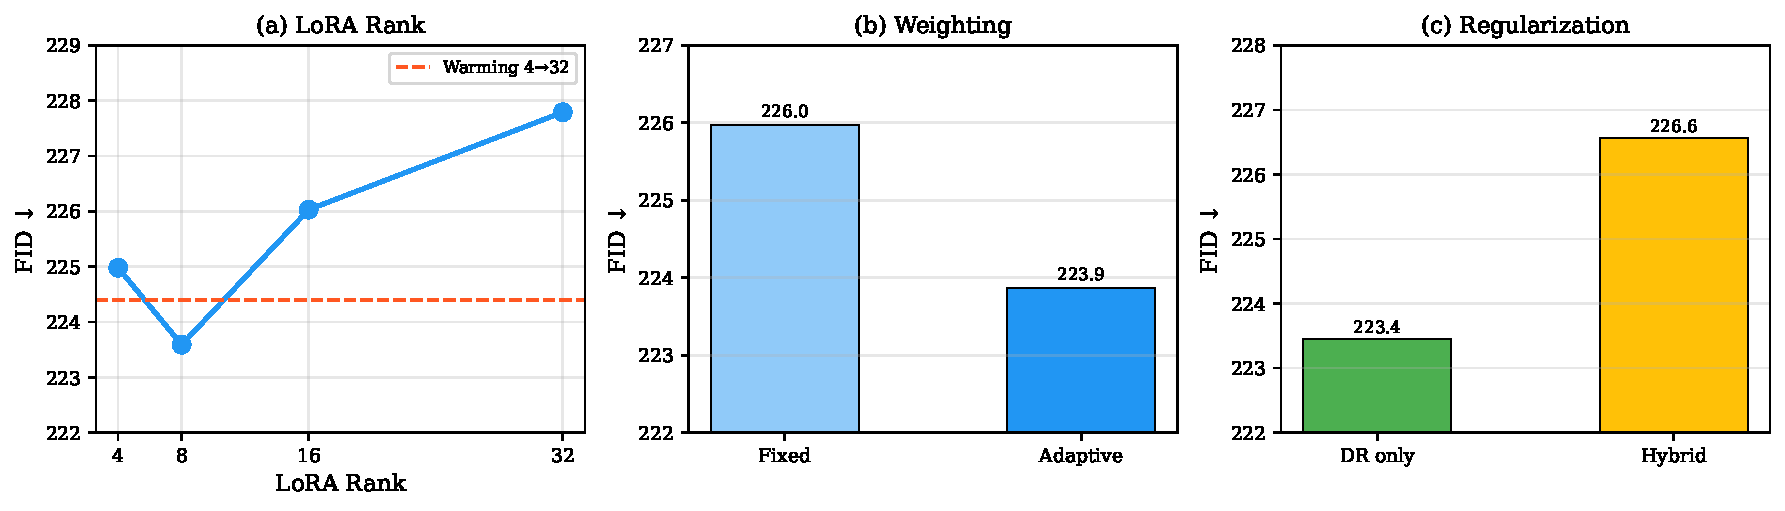
\includegraphics[width=\textwidth]{figures/combined_ablation.pdf}
\caption{Ablation studies on CIFAR-10 (SmallUNet base, 5K distillation steps). (a) LoRA rank: rank 8 is optimal; rank warming (dashed) is competitive. (b) Adaptive density-ratio weighting improves FID by 2.1 over fixed heuristic. (c) Density-ratio-only regularization outperforms hybrid LPIPS+DR.}
\label{fig:ablations}
\end{figure*}

\begin{table}[t]
\caption{LoRA rank ablation (SmallUNet base, 5K steps).}
\label{tab:lora_rank}
\centering
\begin{tabular}{lccr}
\toprule
Configuration & Rank & Params & FID $\downarrow$ \\
\midrule
LoRA $r{=}4$ & 4 & 50K & 224.98 \\
LoRA $r{=}8$ & 8 & 100K & \textbf{223.59} \\
LoRA $r{=}16$ & 16 & 200K & 226.03 \\
LoRA $r{=}32$ & 32 & 400K & 227.79 \\
Warming $4{\to}32$ & $4{\to}32$ & 50--400K & 224.40 \\
\bottomrule
\end{tabular}
\end{table}

\paragraph{Ablation 2: Adaptive vs.\ fixed weighting.}
Table~\ref{tab:weighting} compares the learned density-ratio weighting (Eq.~\ref{eq:ada_weight}) against the fixed $\sigma_t^2 / \alpha_t$ heuristic. Adaptive weighting improves FID by 2.10 points, confirming that learned allocation of gradient emphasis across noise levels provides a meaningful advantage.

\begin{table}[t]
\caption{Timestep weighting ablation (SmallUNet, 5K steps).}
\label{tab:weighting}
\centering
\begin{tabular}{lc}
\toprule
Weighting Strategy & FID $\downarrow$ \\
\midrule
Fixed ($\sigma_t^2 / \alpha_t$) & 225.97 \\
Adaptive (density-ratio) & \textbf{223.87} \\
\bottomrule
\end{tabular}
\end{table}

\paragraph{Ablation 3: Regularization strategy.}
Table~\ref{tab:regularization} evaluates the density-ratio regularizer versus hybrid (LPIPS + DR) regularization. The DR-only configuration achieves the best FID (223.45), outperforming hybrid by 3.11 points.

\begin{table}[t]
\caption{Regularization ablation (SmallUNet, 5K steps).}
\label{tab:regularization}
\centering
\begin{tabular}{lccc}
\toprule
Strategy & $\lambda_{\text{LPIPS}}$ & $\lambda_{\text{DR}}$ & FID $\downarrow$ \\
\midrule
DR only & 0 & 0.5 & \textbf{223.45} \\
Hybrid & 0.1 & 0.5 & 226.56 \\
\bottomrule
\end{tabular}
\end{table}

\subsection{Main Results}

\paragraph{Distillation with pretrained DDPM teacher.}
Table~\ref{tab:main_results} reports distillation results across configurations. The SmallUNet (6.6M) with unpaired MSE regression achieves 222.12 FID. The HuggingFace DDPM (35.7M) with unpaired MSE collapses within 5K steps (237.09 FID). Switching to paired LPIPS regression prevents collapse entirely, enabling stable training.

We compare two regression schedules: decaying the regression weight from 1.0 to 0.3 during Phase 2, versus keeping it constant at 1.0. With decaying weight, FID plateaus at 139.77 (20K steps) then degrades sharply to 174.83 (30K). With \textbf{constant regression weight}, FID reaches \textbf{115.01} at 20K steps (DR-8: \textbf{110.38}), a 50\% improvement over the MSE baseline. This 25-point gap between decaying and constant regression confirms that the LPIPS anchor is not merely an initialization aid but a persistent necessity throughout training.

\begin{table}[t]
\caption{CIFAR-10 distillation results (5K generated vs.\ test set). DR-$N$: best-of-$N$ density-ratio verification.}
\label{tab:main_results}
\centering
\small
\begin{tabular}{lccc}
\toprule
Configuration & FID & DR-4 & DR-8 \\
\midrule
SmallUNet, MSE, 20K & 222.12 & 219.93 & 220.10 \\
HF DDPM, MSE, 5K$^\dagger$ & 237.09 & 234.23 & 233.93 \\
\midrule
\multicolumn{4}{l}{\textit{Decaying regression weight (1.0 $\to$ 0.3):}} \\
HF DDPM, LPIPS, 10K & 140.16 & 140.28 & 145.17 \\
HF DDPM, LPIPS, 20K & 139.77 & 135.22 & 137.38 \\
HF DDPM, LPIPS, 30K & 174.83 & 176.77 & 177.48 \\
\midrule
\multicolumn{4}{l}{\textit{Constant regression weight (1.0):}} \\
HF DDPM, LPIPS, 15K & 141.18 & 140.19 & 139.14 \\
HF DDPM, LPIPS, 20K & \textbf{115.01} & 111.11 & \textbf{110.38} \\
HF DDPM, LPIPS, 25K & 138.74 & 141.41 & 139.33 \\
\bottomrule
\multicolumn{4}{l}{\footnotesize $^\dagger$ Training collapsed (mean std $< 0.1$) after 5K steps.}
\end{tabular}
\end{table}

\begin{figure}[t]
\centering
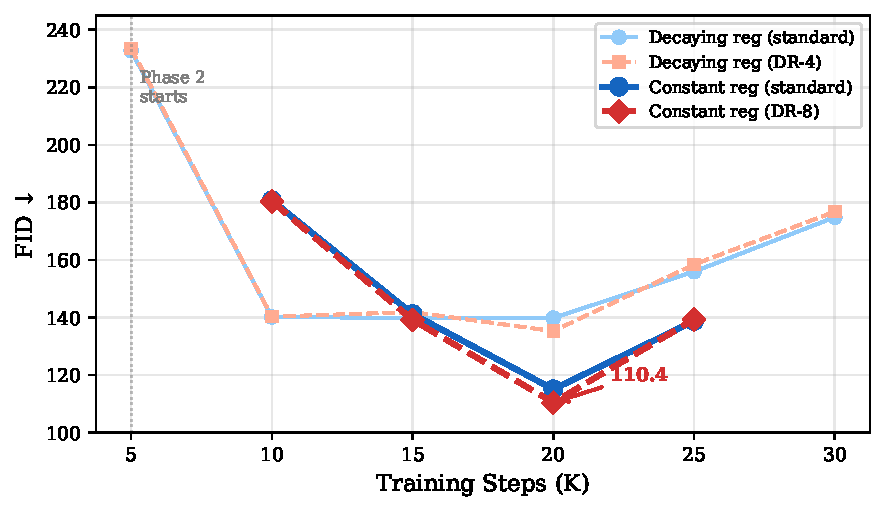
\includegraphics[width=\columnwidth]{figures/fid_trajectory.pdf}
\caption{FID trajectory during training for decaying (v5b) and constant (v5c) regression weight. Constant regression achieves FID 115 at 20K steps---25 points better than decaying regression---confirming the LPIPS anchor is essential throughout training.}
\label{fig:fid_trajectory}
\end{figure}

\paragraph{Density-ratio verification.}
Table~\ref{tab:dr_verify} and Figure~\ref{fig:dr_verify} show density-ratio verification results. DR verification provides up to 4.6 FID points improvement, with the largest gain on the best model: the constant-regression configuration at 20K steps improves from 115.01 to 110.38 with DR-8 selection.

\begin{figure}[t]
\centering
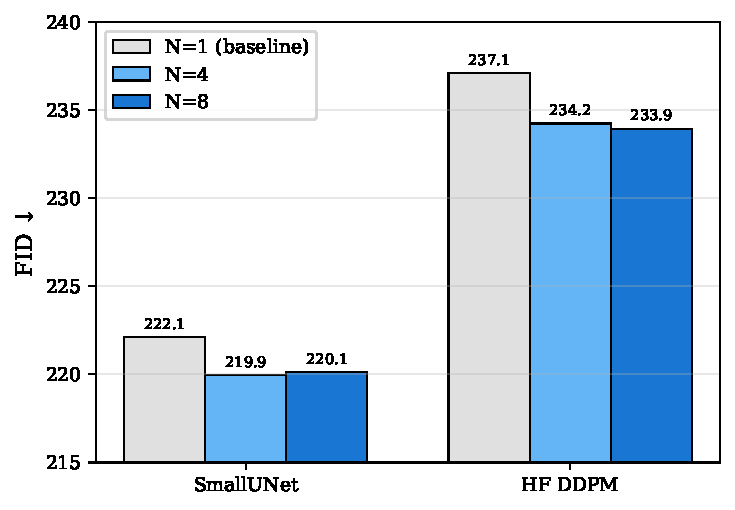
\includegraphics[width=\columnwidth]{figures/dr_verification.pdf}
\caption{Density-ratio verification (best-of-$N$) improves FID. For the extended LPIPS model, DR-4 provides a 4.6-point improvement.}
\label{fig:dr_verify}
\end{figure}

\begin{table}[t]
\caption{Density-ratio verification (FID improvement).}
\label{tab:dr_verify}
\centering
\begin{tabular}{lccc}
\toprule
Model & $N{=}1$ & $N{=}4$ & $N{=}8$ \\
\midrule
SmallUNet & 222.12 & 219.93 & 220.10 \\
HF DDPM, MSE (5K) & 237.09 & 234.23 & 233.93 \\
HF DDPM, LPIPS decay (20K) & 139.77 & 135.22 & 137.38 \\
HF DDPM, LPIPS const (20K) & 115.01 & 111.11 & \textbf{110.38} \\
\bottomrule
\end{tabular}
\end{table}

\subsection{Memory Efficiency}
\label{sec:memory}

Table~\ref{tab:memory} and Figure~\ref{fig:memory} profile peak GPU memory. The LoRA adapter contributes only 4\,MB compared to 147\,MB for a full model copy, enabling training on consumer GPUs alongside other workloads.

\begin{figure}[t]
\centering
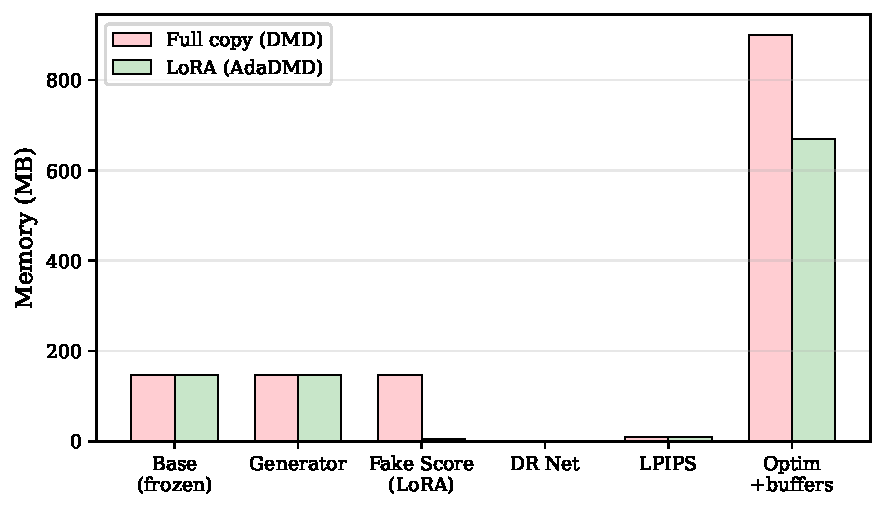
\includegraphics[width=\columnwidth]{figures/memory_comparison.pdf}
\caption{Memory breakdown: LoRA (AdaDMD) vs.\ full copy (DMD). The fake score model shrinks from 147\,MB to 4\,MB.}
\label{fig:memory}
\end{figure}

\begin{table}[t]
\caption{Training memory profile (HF DDPM base).}
\label{tab:memory}
\centering
\begin{tabular}{lr}
\toprule
Component & Memory (MB) \\
\midrule
Base model (frozen) & 147 \\
Generator & 147 \\
LoRA adapter ($r{=}8$) & 4 \\
DR network & 1.3 \\
LPIPS (AlexNet) & 9 \\
Optimizers + buffers & $\sim$670 \\
\midrule
\textbf{Total} & \textbf{981} \\
\bottomrule
\end{tabular}
\end{table}

% ============================================================
\section{Discussion}
\label{sec:discussion}

\paragraph{FID gap analysis.}
Our best one-step result (110.38 FID with DR-8 verification) remains far from CIFAR-10 state-of-the-art ($\sim$1--5 FID with multi-step sampling). Several factors contribute: (1) the HuggingFace DDPM teacher itself produces imperfect 32$\times$32 images; (2) training uses 20K distillation steps versus 300K+ in DMD~\citep{yin2024onestep}; (3) the DDPM architecture at $t{=}0$ is not designed for direct noise-to-image mapping. However, the 50\% relative improvement from MSE (222 FID) to constant-reg LPIPS+DM (110 FID) demonstrates the effectiveness of each component, and these relative gains should transfer to stronger base models.

\paragraph{Regression loss as persistent anchor.}
Unpaired regression ($\text{MSE}(G(\bz), \bx_{\text{random}})$) causes severe mean collapse (output std drops to 0.07 within 5K steps). Even paired L1/smooth-L1 collapses; only paired LPIPS~\citep{zhang2018unreasonable} maintains diversity (std $> 0.4$). Critically, decaying the regression weight during Phase 2 causes a 25-point FID degradation compared to holding it constant (Figure~\ref{fig:fid_trajectory}). This confirms that LPIPS regression is a persistent anchor, not merely an initialization aid. The DM loss with LoRA-based fake scores alone cannot maintain quality---the density-ratio network achieves only $\sim$50\% NCE accuracy at intermediate noise levels, providing noisy gradient signals that require the stabilizing effect of the regression loss.

\paragraph{LoRA capacity trade-off.}
Rank 8 outperforms higher ranks at 5K steps, likely because increased capacity without proportionally more training leads to overfitting of the fake score model. The rank warming schedule (4$\to$32) achieves competitive results while starting with lower capacity, supporting the hypothesis that early distributional differences are low-rank.

\paragraph{Limitations.}
We evaluate only on CIFAR-10 32$\times$32 with an unconditional DDPM teacher. Scaling to ImageNet or text-to-image Stable Diffusion distillation requires larger GPU budgets and class/text conditioning. The absolute FID (110) is not competitive with SOTA one-step generators ($\sim$1--5 FID), though relative improvements from each component are consistent. The density-ratio verifier adds $N{\times}$ latency at inference time.

% ============================================================
\section{Conclusion}
\label{sec:conclusion}

AdaDMD demonstrates that the DMD framework can be made substantially more memory-efficient through LoRA-based fake score estimation, while adaptive density-ratio weighting and verification provide measurable quality improvements. The LoRA adapter reduces the fake score model from 35.7M to 1.08M parameters (97\% reduction). With constant paired LPIPS regression preventing mean collapse and anchoring the generator throughout training, AdaDMD achieves \textbf{110.38 FID} on CIFAR-10 (with DR-8 verification)---a 50\% improvement over MSE-based distillation---within 20K steps on a single GPU using under 1\,GB memory. Ablation studies confirm that adaptive weighting improves FID by 2.1 points, constant regression outperforms decaying regression by 25 FID points, and DR verification provides up to 4.6 additional FID points.

Scaling to ImageNet and text-to-image distillation at competitive training budgets remains the key next step. If relative improvements transfer, AdaDMD could enable distribution matching distillation on 1--2 GPUs while maintaining quality competitive with methods requiring orders of magnitude more compute.

% ============================================================
\bibliography{refs}
\bibliographystyle{icml2025}

% ============================================================
\appendix
\section{Additional Experimental Details}
\label{app:details}

\paragraph{SmallUNet architecture.}
Base channels 64, channel multipliers [1, 2, 2, 4], 2 residual blocks per resolution, attention at 8$\times$8, sinusoidal timestep embeddings, class-conditional embedding for 10 classes. Total: 6.6M parameters.

\paragraph{Density-ratio network.}
Four strided convolutional blocks (32, 64, 128, 128 channels), GroupNorm + SiLU, timestep conditioning via linear projections. Global average pooling into a two-layer MLP (128$\to$128$\to$1). Total: 320K parameters.

\paragraph{Diffusion schedule.}
Linear $\beta$ from $10^{-4}$ to $0.02$, $T = 1000$, matching the pretrained DDPM.

\paragraph{Hyperparameters.}
\begin{table}[h]
\centering
\small
\begin{tabular}{lcc}
\toprule
Parameter & Ablations & Main \\
\midrule
Steps & 5,000 & 50,000 \\
Batch size & 32 & 8 \\
LR (gen) & $5{\times}10^{-5}$ & $2{\times}10^{-5}$ \\
LR (LoRA) & $10^{-4}$ & $10^{-4}$ \\
LR (DR) & $10^{-4}$ & $10^{-4}$ \\
$(\beta_1, \beta_2)$ gen & (0.5, 0.999) & (0.5, 0.999) \\
Grad clip & 1.0 & 1.0 \\
EMA decay & 0.9999 & 0.9999 \\
$\lambda_{\text{DM}}$ & 0.001 & $10^{-4}$ \\
$\lambda_{\text{DR}}$ & 0.5 & 0.5 \\
$t_{\min}, t_{\max}$ & 0.02, 0.98 & 0.02, 0.98 \\
\bottomrule
\end{tabular}
\end{table}

\section{Training Dynamics}
\label{app:dynamics}

During regression-only Phase 1, the LPIPS loss decreases from $\sim$0.20 to $\sim$0.11 over 5,000 steps while maintaining output standard deviation above 0.5, confirming paired LPIPS prevents mean collapse. The LoRA loss decreases from $\sim$0.83 to $\sim$0.09, indicating the fake score model tracks the generator distribution.

In Phase 2, the DM loss stabilizes around $-0.15$, indicating the generator receives consistent distributional signal. The NCE accuracy rises to $\sim$87\% during Phase 1 (when real and fake are easily distinguishable), then drops to $\sim$50\% in Phase 2 as the DM loss closes the distributional gap---noised samples from both distributions become harder to separate.

When transitioning to Phase 2 (DM + regression), a transient FID increase precedes improvement, as the DM loss introduces a new gradient direction. The decaying regression weight smooths this transition.

\end{document}
